% !TeX spellcheck = en_US
% !TeX encoding = UTF-8

% COMPILE WITH:
% `latexmk`
% You need lualatex and biber (in all TeXLive distributions)

\documentclass[
    numbers=noenddot,
    %listof=totoc,
    parskip=half-,
    fontsize=12pt,
    paper=a4,
    oneside,
    titlepage,
    bibliography=totoc,
    chapterprefix=false,
%    draft
]{scrbook}

% use lualatex or xelatex
\usepackage{fontspec}
\usepackage{graphicx}
\usepackage[doublespacing]{setspace}

% better language support
\usepackage{polyglossia}
\setdefaultlanguage{english}
\setotherlanguage{german}

\usepackage{hyperref}
\usepackage{tocbasic}
\usepackage{booktabs}
\usepackage{multicol}
\usepackage{multirow}

\usepackage[]{scrlayer-scrpage}

% better bibliography (biblatex style)
% use biber to compile
\usepackage[citestyle=alphabetic, bibstyle=alphabetic, sorting=nyt, backend=biber, language=english, backref=true, maxcitenames=2]{biblatex}

% better quotes
% use \enquote{text}
\usepackage[autostyle,english=american,german=quotes]{csquotes}
\usepackage{listings}
\addbibresource{bibliography.bib}

% appendix
\usepackage[titletoc]{appendix}

% where to put all images and figures
\graphicspath{{images/}}

% YOUR PACKAGES


% Title
\title{Second Lab - Creating LSTM Model}

% Author
\author{Sayed Alisina Qaderi, Atiqullah Ahmadzai \& Dusan Dordevic}

% Date
\date{\today}

% CHOOSE ACCORDINGLY
%\newcommand{\thesisType}{Bachelorarbeit}
\newcommand{\thesisType}{MasterLab}

\makeatletter
\let\thetitle\@title
\let\theauthor\@author
\let\thedate\@date
\makeatother

\pagestyle{scrheadings}

\begin{document}

%%%%%%%%%%%%%%%%%%%%%%%%%%%%%%%%%%%%%%%%%%%%%%%%%%%%%%%%%%%%%%%%%%%%%%%%%%%%%%%%%%%%%%%%%
\frontmatter
% CHOOSE ACCORDINGLY
%% !TeX spellcheck = en_US
% !TeX encoding = UTF-8
\begin{titlepage}
    \centering
    \begin{onehalfspace}
    	\begin{german}
        	
\includegraphics[width=7cm]{uni-logo.png}\\
        	\vspace{1.0cm}
        	\large {\bfseries Lehrstuhl für Informatik mit Schwerpunkt\\ \textenglish{Digital Libraries and Web Information Systems}} \\

        	\vspace{2.5cm}

            \begin{doublespace}
            	\textenglish{\textsf{\Huge{\thetitle}}}
            \end{doublespace}

        	\vspace{2cm}

            \Large{Bachelorarbeit von}\\

        	\vspace{1cm}

        	{\bfseries \large{\theauthor}}

        	\vfill

        	{\large
        		\begin{tabular}[l]{cc}
        			\textsc{Prüfer}\\
        			Prof.~Dr.~Siegfried Handschuh
        		\end{tabular}
        	}

        	\vspace{1.5cm}

        	\parbox{\linewidth}{\hrule\strut}

            \vfill

	    \textgerman{\thedate}
    	\end{german}
    \end{onehalfspace}
\end{titlepage}

% !TeX spellcheck = en_US
% !TeX encoding = UTF-8
\begin{titlepage}
    \centering
    \begin{onehalfspace}
    	\begin{german}
        	
\includegraphics[width=7cm]{uni-logo.png}\\
        	\vspace{1.0cm}
        	\large {\bfseries Security Insider Lab II}\\ 

        	\vspace{2.5cm}

            \begin{doublespace}
            	\textenglish{\textsf{\Huge{\thetitle}}}
            \end{doublespace}

        	\vspace{2cm}
    
            

        	\vspace{1cm}

        	{\bfseries \large{\theauthor}}

        	\vfill

        	% {\large
        	% 	\begin{tabular}[l]{cc}
        	% 		\textsc{1.} & \textsc{2.~xxxxx} \\
        			
        	% 	\end{tabular}
        	% }

        	\vspace{1.5cm}

        	\parbox{\linewidth}{\hrule\strut}

            \vfill

	    \textgerman{\thedate}
    	\end{german}
    \end{onehalfspace}
\end{titlepage}


\tableofcontents
\newpage

% -- ABSTRACT
% % !TeX spellcheck = en_US
% !TeX encoding = UTF-8
\chapter*{Abstract}
The Vulnerability Scanner project aims to enhance software security by developing a tool that identifies and reports security vulnerabilities within software projects. 
The tool provides functionalities for user authentication, project creation, and management, as well as the capability to scan code repositories or Python source files for various vulnerabilities. 
By leveraging advanced machine learning models, including LSTM and GPT API the system detects vulnerabilities and generates comprehensive reports. 
Users can rescan their code after implementing fixes to ensure improved security. 
The system architecture includes a user-friendly interface, a robust backend for service management, a secure database for storing credentials and project data, and pre-trained machine learning models for effective vulnerability detection. 
The workflow involves user login, project setup, code retrieval and conversion, vulnerability analysis, report generation, and rescanning. 
This approach ensures a continuous cycle of security assessment and improvement, addressing vulnerabilities such as XSS, Path Disclosure, Remote Code Execution, and Command Injection.
% \newpage

% % -- Acknowledgements (optional)
% % !TeX spellcheck = en_US
% !TeX encoding = UTF-8
\chapter*{Acknowledgments}

% I would first like to thank my thesis advisor ...
% \newpage

% -- List of figures
\thispagestyle{empty}
\cleardoublepage
\listoffigures
\newpage

% % -- List of tables
% \thispagestyle{empty}
% \cleardoublepage
% \listoftables
% \newpage

%%%%%%%%%%%%%%%%%%%%%%%%%%%%%%%%%%%%%%%%%%%%%%%%%%%%%%%%%%%%%%%%%%%%%%%%%%%%%%%%%%%%%%%%%
\mainmatter

% -- Chapters
% following IMRaD structure
% adjust for your liking
\chapter{Introduction}\label{chap:introduction}

The SafeScript project addresses the critical need for enhanced security in software development by developing an advanced tool that identifies security vulnerabilities within software projects. 
This project aims to provide users with comprehensive capabilities to log in, create, and manage projects, and scan code repositories or Python source files for various vulnerabilities. 
The system employs sophisticated machine learning models to detect potential security issues and generates detailed reports. 
Additionally, users can rescan their code after making necessary fixes to ensure that security improvements are effectively implemented.

The project encompasses several functional requirements. 
First, it includes a user authentication feature where users must log in with a username and password to access the system, ensuring secure access. 
Second, it allows for project creation, enabling users to create new projects by providing a name and selecting a code repository or uploading a Python source code file. 
Third, repository management lets users specify the source of the code, either via a repository link or direct file upload. 
Fourth, the code retrieval function automates the process of fetching the code from the specified repository or processing the uploaded file. 
Fifth, data conversion converts the retrieved code into word2vec (w2v) format for subsequent vulnerability analysis. 
Sixth, vulnerability detection utilizes pre-trained machine learning models (LSTM, ChatGPT API) to identify vulnerabilities in the code. 
Seventh, report generation produces a comprehensive report detailing detected vulnerabilities, their severity, and recommendations for remediation. 
Eighth, the rescan capability allows users to rescan their code post-fix to confirm that vulnerabilities have been addressed. 
Lastly, the system supports the detection of specific types of vulnerabilities, including XSS (Cross-Site Scripting), Path Disclosure, Remote Code Execution, and Command Injection.

The technical architecture of the SafeScript system comprises several key components. 
The user interface (UI) includes a login page, a dashboard for project management, and options for report viewing and rescanning. 
The backend includes services for authentication, project management, code retrieval, vulnerability detection, and report generation. 
The database stores user credentials, project details, and scanning results and reports. 
The system also incorporates pre-trained machine learning models (LSTM and ChatGPT API) for vulnerability detection.

The workflow of the SafeScript system involves several steps. Initially, the user logs in using credentials. 
The user then creates a new project and selects the source of the code. 
The system fetches the code from the repository or processes the uploaded file. 
The code is then converted to w2v format, and the selected machine learning model analyzes the code for vulnerabilities. 
Subsequently, the system generates and displays a report. Finally, the user can rescan the code after making fixes to ensure that vulnerabilities have been addressed.
Figure \ref{fig:workflow} shows the complete workflow of the applications.

\begin{figure}[H]
    \centering
    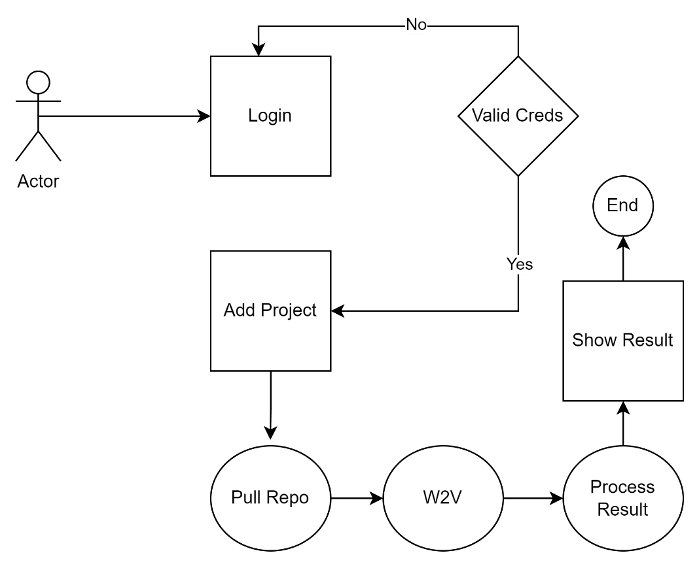
\includegraphics[width=0.9\linewidth]{images/workflow.png}
    \caption{SafeScript workflow diagram}
    \label{fig:workflow}
\end{figure}

This structured approach ensures that the system not only identifies security vulnerabilities effectively but also facilitates continuous improvement in code security through iterative scans and fixes.
\chapter{Methods}\label{chap:methods}

\subsection{Data Collection}

We initiated the data collection process by scraping GitHub repositories. 
Utilizing web scraping techniques, we gathered data from 2000 repositories, encompassing a diverse range of projects. 
The default amount of repositories was 100000, which is a considerable amount. 
Considering our time constraints and the need for a more efficient process, we made the decision to change the default steps to 2000, keeping you informed and involved in the process. \ref{fig:srapingLabel}

As we worked on \textbf{scrapingGithub.py} file, we have faced the following issues. The solutions are also mentioned in below:
\begin{itemize}
    \item Missing \textbf{requests} library solved with \textit{ pip install requests }
    \item Missing \textbf{requests\_oauthlib} library, solved with  \textit{pip install requests\_oauthlib}
    \item Missing \textbf{all\_commits} file which we created manually.
    \item Missing Github Access Token, we generated through Github and save to \textbf{access} file inside the project folder. 
    \item Requests needed exception handling in case of losing the network.
\end{itemize}

After solving the above issue, they successfully ran the \textbf{scrapingGithub.py}, and its results were saved in \textbf{allcommits.json} file.

\begin{figure}
    \centering
    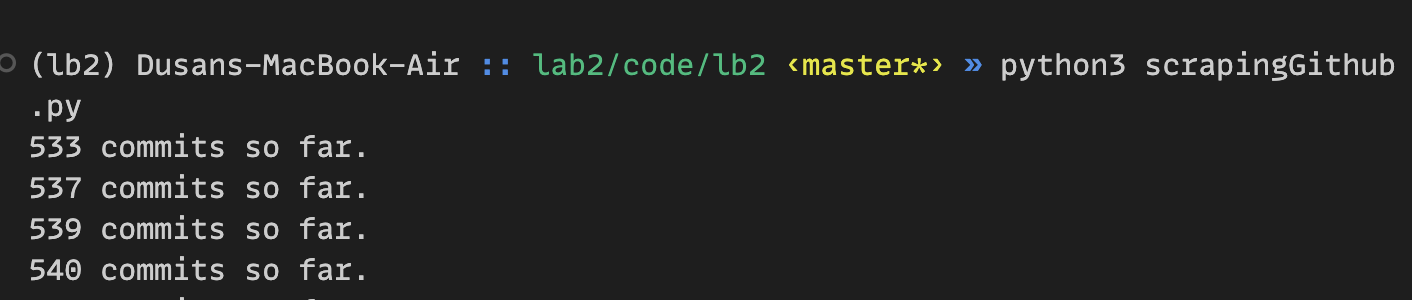
\includegraphics[width=0.5\linewidth]{Screenshot 2024-05-12 at 10.42.04.png}
    \caption{Gathering repositories}
    \label{fig:srapingLabel}
\end{figure}


\subsection{Keyword Filtering}

Following data collection, we performed keyword filtering to refine the dataset with \textbf{filterShowcase.py} file. 
By examining the names and readme files of the scraped repositories, we identified and filtered out repositories that matched our predefined keywords.
We have filtered the following showcases:
\begin{itemize}
    \item toomuchsecurity = ['offensive', 'pentest', 'vulnerab', 'security', 'hack', 'exploit', 'ctf ', ' ctf', 'capture the flag','attack'] 
    \item alittletoomuch = ['offensive security', 'pentest', 'exploits', 'vulnerability research', 'hacking', 'security framework', 'vulnerability database', 'simulated attack', 'security research'] 
    \end{itemize}

\subsection{Language Segregation}

With the help of \textbf{getDiffs.py} class file, we refined the dataset by segregating libraries with Python code from those without. 
This step was crucial for our subsequent analysis, focusing specifically on repositories containing Python code.
During this process, we faced the following issues:

\begin{itemize}
    \item missing os library which resolved by \textit{import os} \ref{fig:diff_os}.
    \item \textbf{datata} typo in line 110, which resolved by changing to \textbf{data} \ref{fig:diff_typo}.
\end{itemize}

\begin{figure}
    \centering
    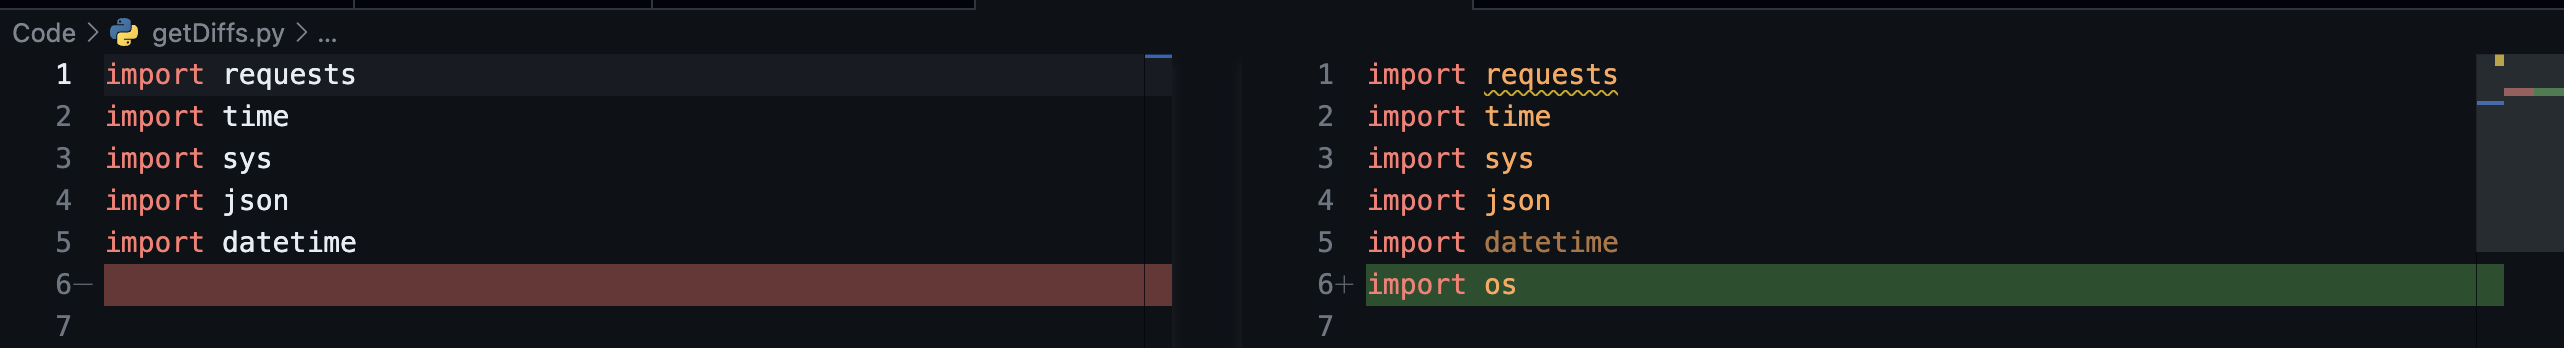
\includegraphics[width=1\linewidth]{getDiffe_os.png}
    \caption{GetDiffs missing os}
    \label{fig:diff_os}
\end{figure}

\begin{figure}
    \centering
    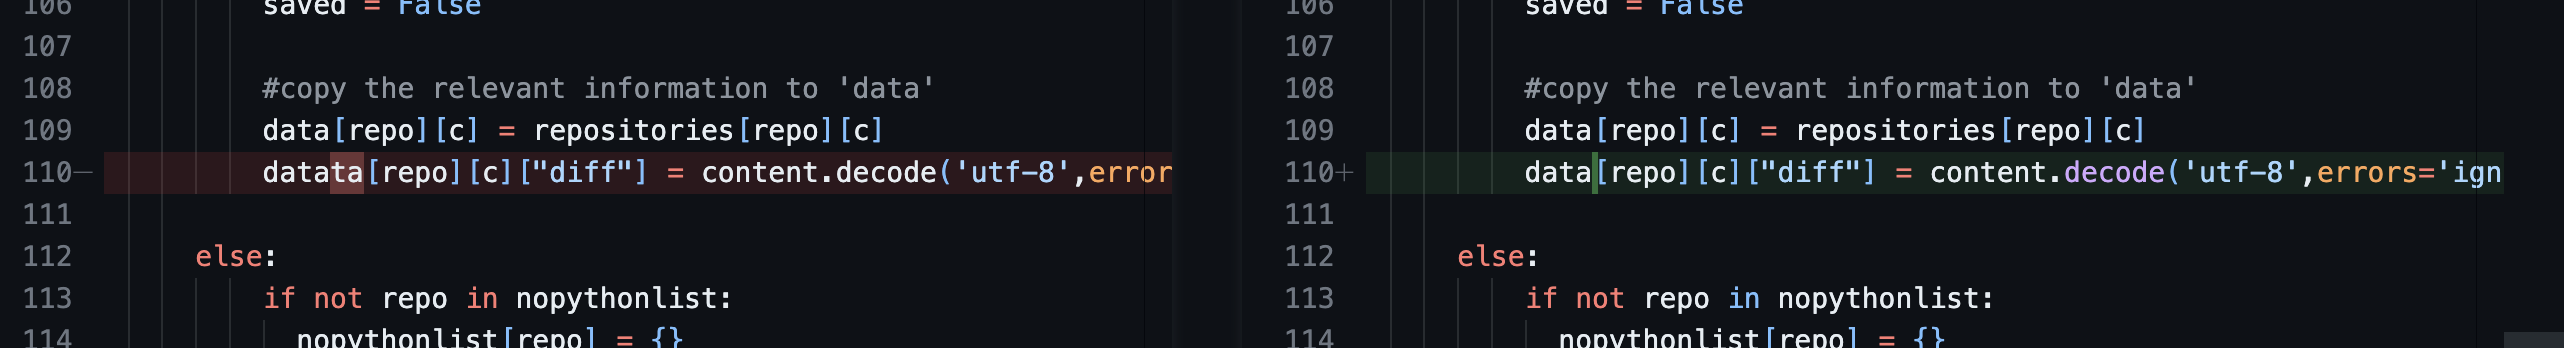
\includegraphics[width=1\linewidth]{getDiffs_typo.png}
    \caption{GetDiffs typo issue}
    \label{fig:diff_typo}
\end{figure}

\subsection{Commit Analysis}

In this step, we meticulously analyzed and downloaded the commits of the filtered repositories with the help of the \textbf{getData.py} file. 
By extracting all differences from their commits, we gained insights into the projects' evolution and the changes made over time.
We faced with only one issue in this phase \textit{ModuleNotFoundError: No module named 'keras.layers.convolutional'} which resolved by \textit{pip install keras} and the rest of code worked ideally and saved the result in \textbf{PyCommitsWithDiffs.json} JSON file.

\subsection{Dataset Acquisition}

To augment our dataset, we procured additional data from the main repository. 
This supplementary dataset, provided by the main repository, was essential for enhancing the depth and scope of our analysis in subsequent stages.

\subsection{Model Training}

The final step involved training our model based on the augmented dataset acquired in the previous step. This step handled with the help \textbf{makemodel.py}.
The Python script is a machine learning pipeline for training and evaluating an LSTM (Long Short-Term Memory) model for identifying vulnerabilities. 
We have trained the model over four types of vulnerabilities, XSS (Cross-Site Scripting), Path Disclosure, Remote Code Execution. The model specification 
is 10 for minimum count, 200 for iterations, 300 for vector size.

While working with this script we have faced the following issues due to library deprecations and changes in the Python version:

\begin{enumerate}

    \item \textbf{Sklearn.util class\_weight} issue which the input parameters changed in the latest verions. The differences shown in the figure \ref{fig:sklearn_class_wight}.
    \item \textbf{AttributeError: The vocab attribute was removed from KeyedVector in Gensim 4.0.0.}, the solution is changing vocab to \textbf{key\_to\_index}.
    \item \textbf{vector = w2v\_model[t] 'Word2Vec' object is not subscriptable} resolved by changing \textit{w2v\_model} to \textit{m2v\_model.wv}.
    \item \textbf{yhat\_classes = model.predict\_classes(X\_train, verbose=0)} issue because of the ... add in here . 
    Therefore we have changed to the \textbf{predict=model.predict(X\_train) yhat\_classes=numpy.argmax(predict,axis=1)}. 
    The final result for this changes shown in figure \ref{fig:yhat_changes}.
    % MARK: talk with atiq about it
    \item \textbf{numpy.core.\_exceptions.\_arraymemoryerror: unable to allocate 2.42 gib for an array with shape (8277, 131, 300) and data type float64} memory issue, we solved this issue with increasing virtual memory to 150 GB and GPU with the help of Tensorflow GPU library.

\end{enumerate}

Figures \ref{fig:makemodel1}, \ref{fig:makemodel2} and \ref{fig:makemodel3} log of each step for execution of this step. 

MARK TODO: Talk Abount the code enhancemnt you have and check if I miss something with ATIQullah

\begin{figure}
    \centering
    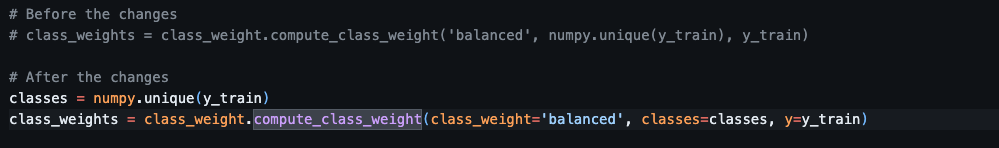
\includegraphics[width=1\linewidth]{sk-classweight.png}
    \caption{Sklearn Utils Class Weight}
    \label{fig:sklearn_class_wight}
\end{figure}

\begin{figure}
    \centering
    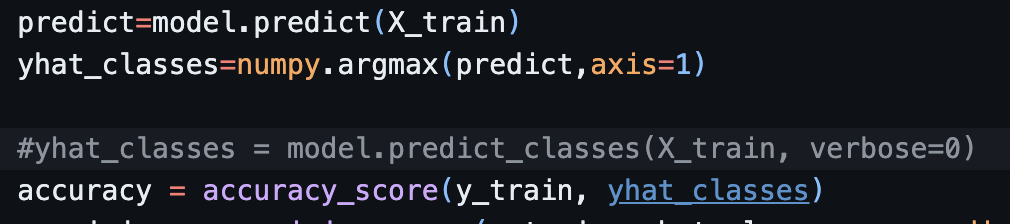
\includegraphics[width=1\linewidth]{yhat_changes.png}
    \caption{Yhat Changes}
    \label{fig:yhat_changes}
\end{figure}

\begin{figure}
    \centering
    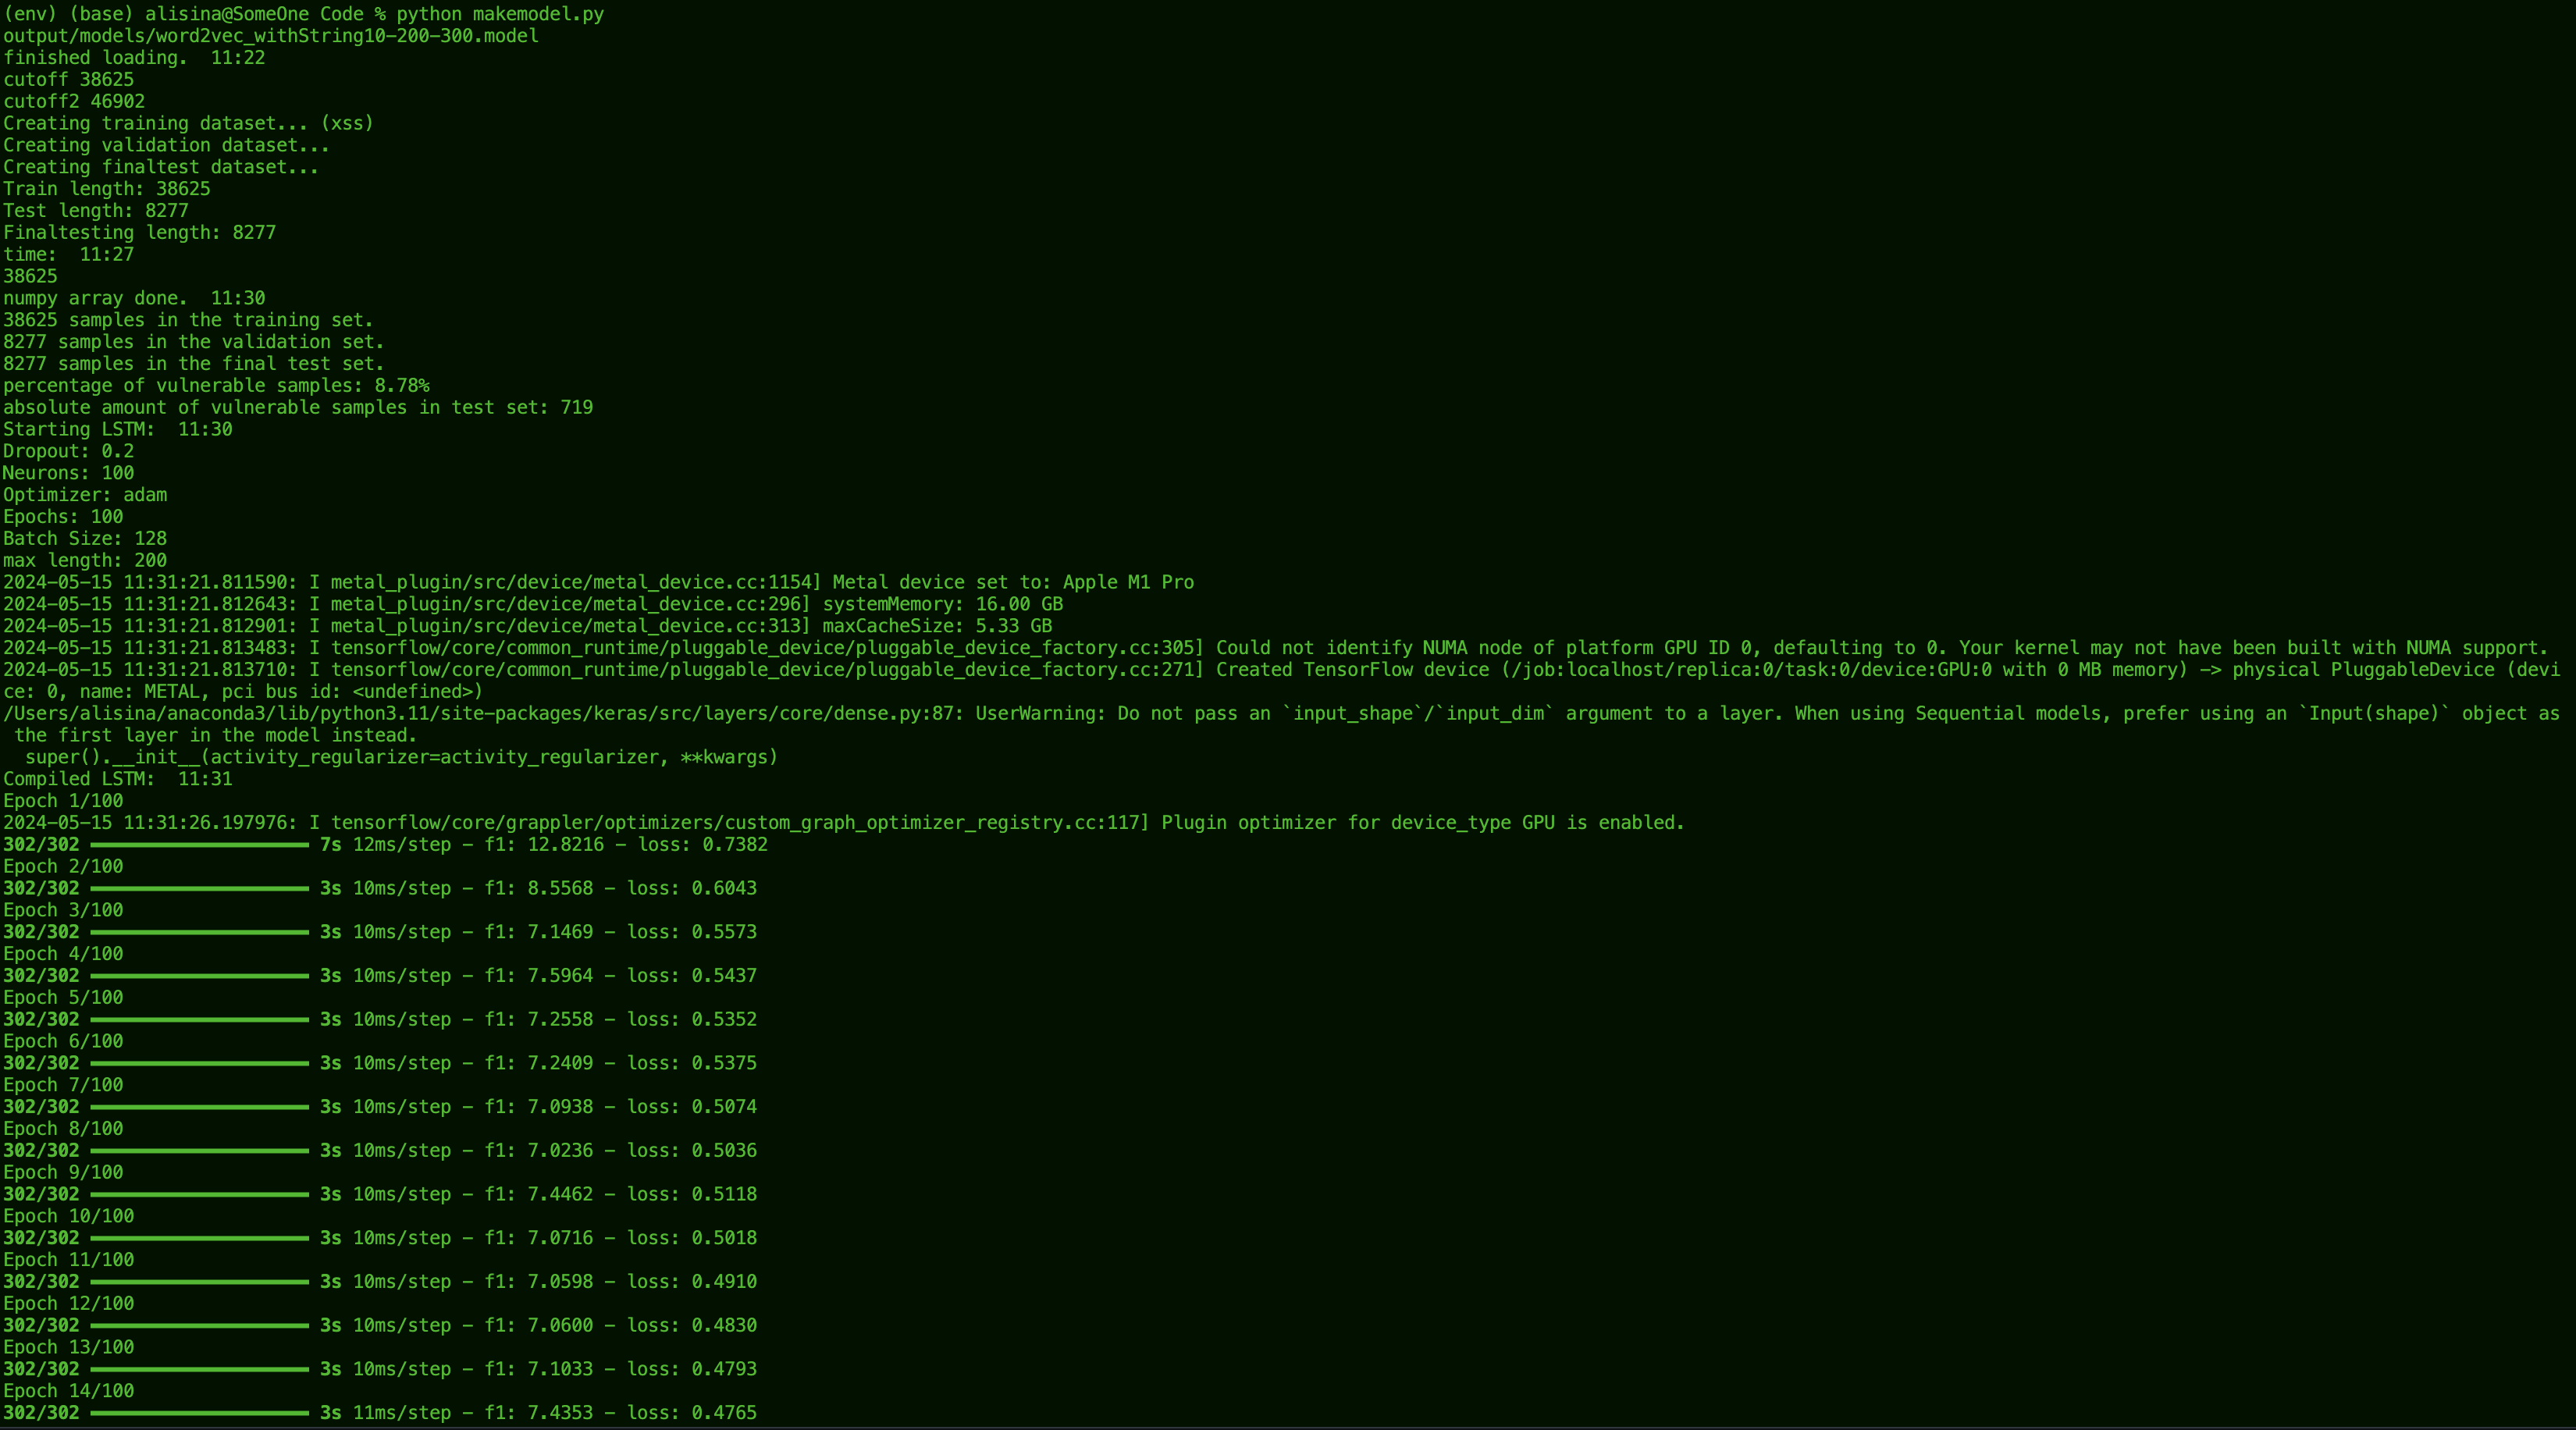
\includegraphics[width=1\linewidth]{makemodel1.png}
    \caption{Loading Data, Filtering Array \& Perpairing Data}
    \label{fig:makemodel1}
\end{figure}

\begin{figure}
    \centering
    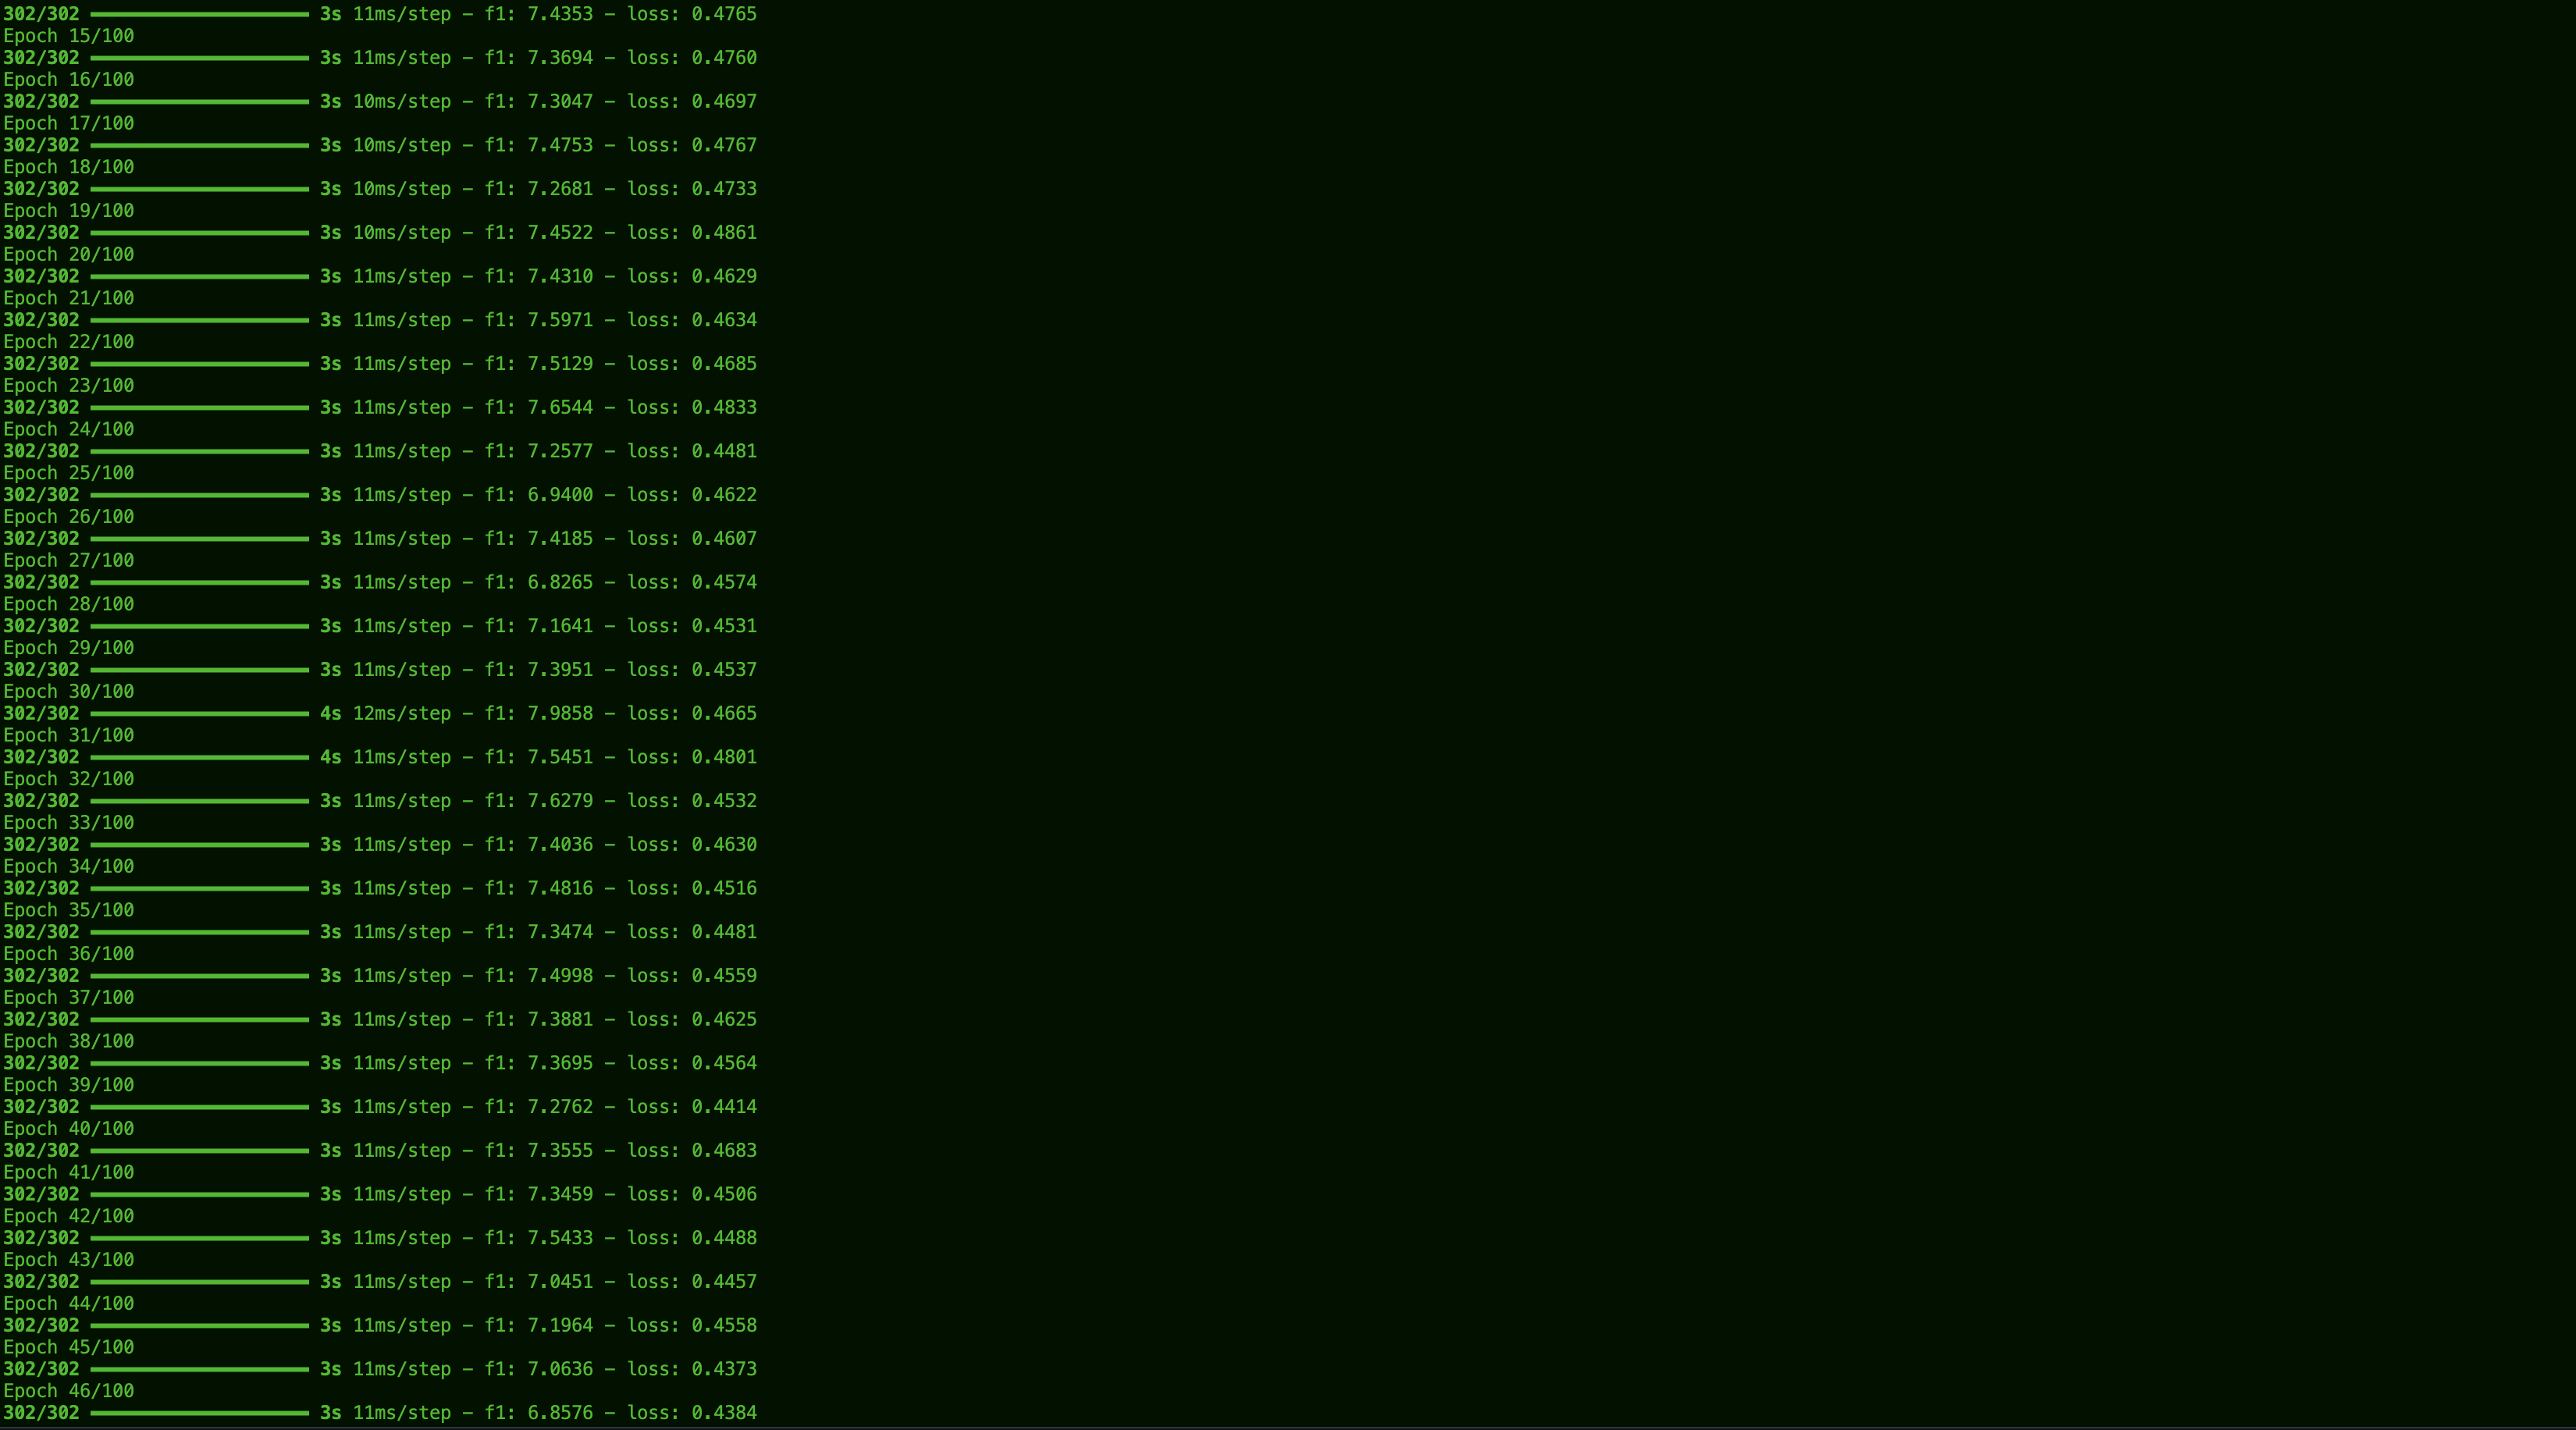
\includegraphics[width=1\linewidth]{makemodel2.png}
    \caption{The Epoch Steps Calculation}
    \label{fig:makemodel2}
\end{figure}
\begin{figure}
    \centering
    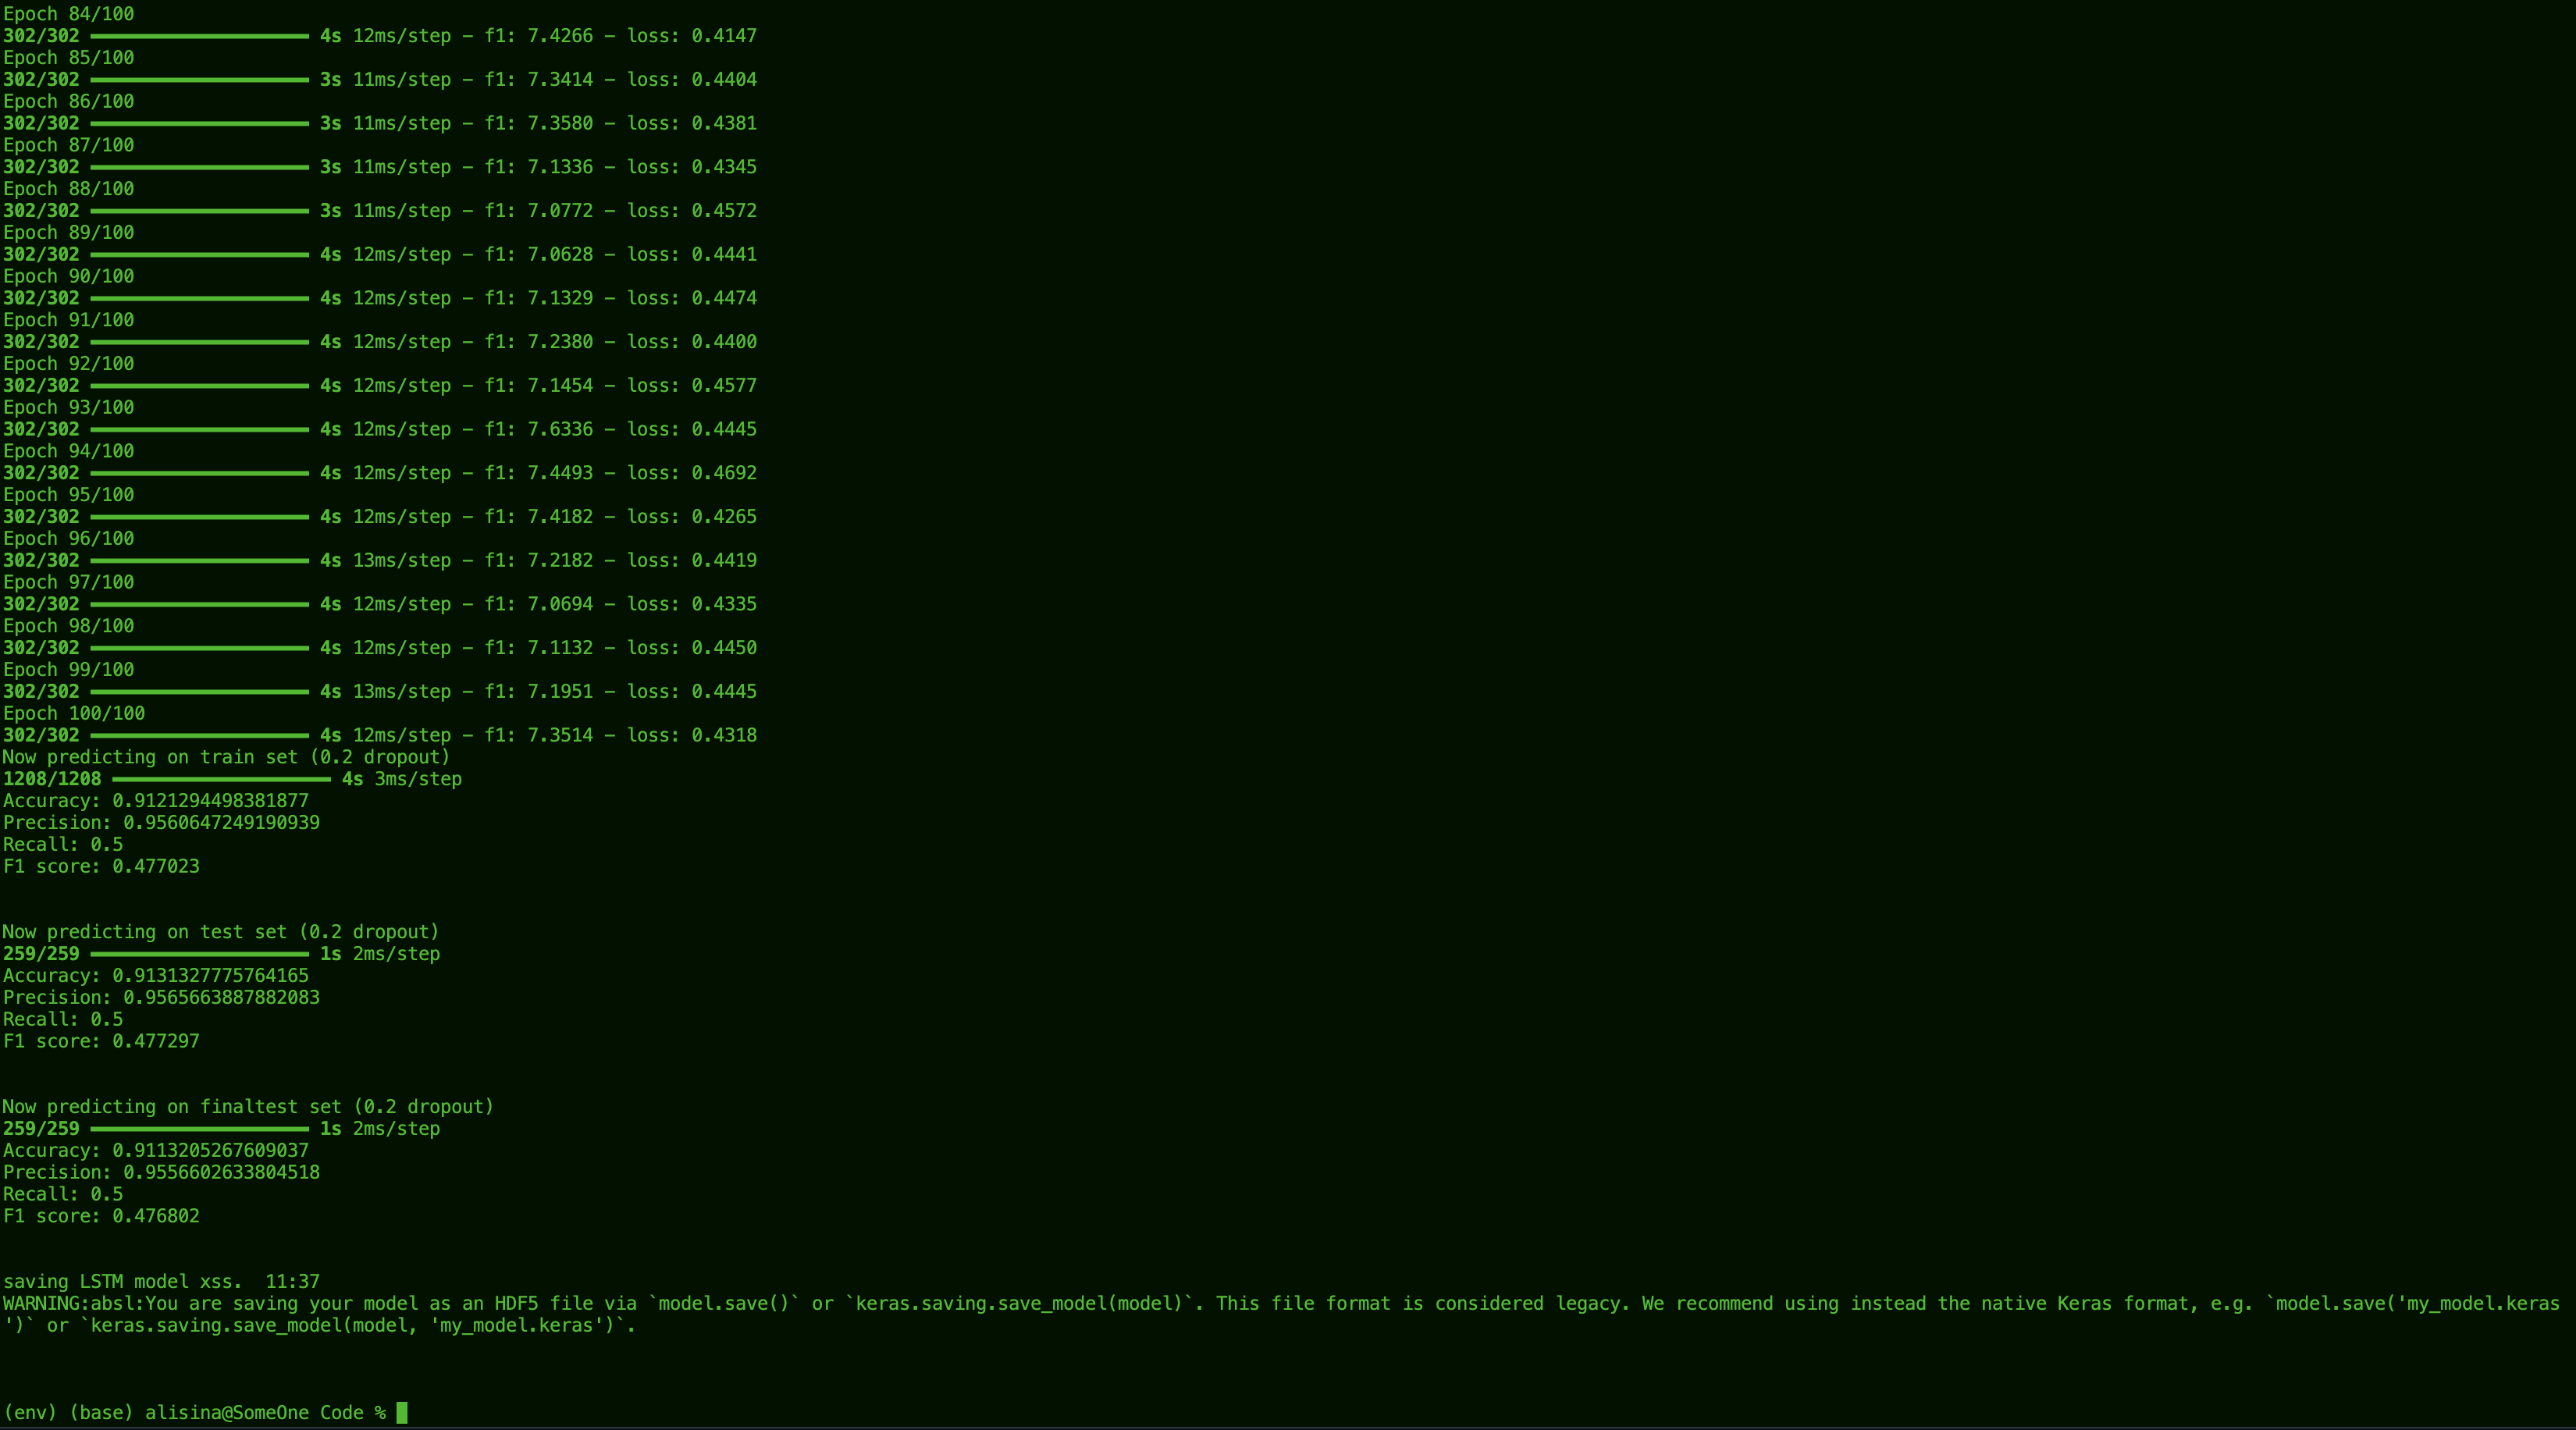
\includegraphics[width=1\linewidth]{makemodel3.png}
    \caption{Model Generation and Saving it}
    \label{fig:makemodel3}
\end{figure}

\chapter{Results}\label{chap:results}

\chapter{Discussion}\label{chap:discussion}


\subsection{\textbf{Creating the LSTM models}}
% We do not need this because, it wan belongs to first lab.


   \textbf{Makemodel.py} script is used for creating data models. It splits the data in 3 different segments (train, validate, final).
   On the line of code 134, the samples are randomized with \textbf{for} loop. However, there are certain issues regarding this code. 
   Library \textbf{Keras} that is imported in myutils.py file is causing a build error. 
   Keras package is now \textbf{included} in previous installation of tensorflow package. 
   Therefore, imports needed to be adjusted accordingly. 
   "from keras.datasets import imdb" is now "tensorflow.keras.datasets". 
   Also, we need to install all necessary packages (gensim, sklearn, tensorflow). 
   Next, datasets are created using word2vec models created in previous exercise. 
   Unfortunately, new error occurs where we need to adjust 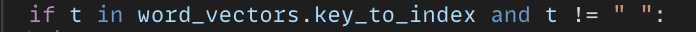
\includegraphics[width=0.5\linewidth]{Screenshot 2024-05-12 at 13.10.36.png} this line of code to match the new key to index parameter. 
   Console is clear from errors so we can proceed to make our new vulnerability model. 
   After loading the data, script creates new training dataset 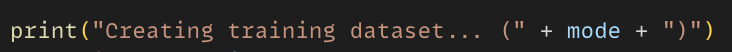
\includegraphics[width=0.5\linewidth]{Screenshot 2024-05-12 at 13.14.57.png}, followed by 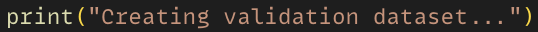
\includegraphics[width=0.5\linewidth]{Screenshot 2024-05-12 at 13.16.00.png} and finally 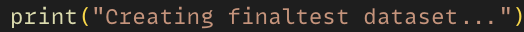
\includegraphics[width=0.5\linewidth]{Screenshot 2024-05-12 at 13.16.43.png}.
                 
   
   %   \begin{figure}
   %     \centering
   %     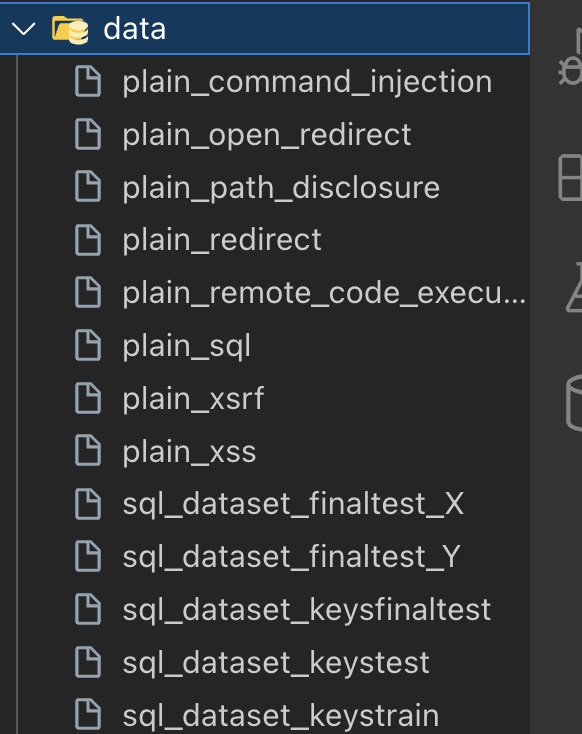
\includegraphics[width=0.5\linewidth]{Screenshot 2024-05-12 at 12.41.42.png}
   %     \caption{Folder structure with data}
   %     \label{fig:enter-label}
   % \end{figure}                               


  % add the console output of final steps
  % adjust the images
  % format the document 
   
   

% -- Appendix (optional)
\begin{appendices}
    % !TeX spellcheck = en_US
% !TeX encoding = UTF-8
% \chapter{Code}

% \chapter{Math}

% \chapter{Dataset}
\end{appendices}
\newpage


%%%%%%%%%%%%%%%%%%%%%%%%%%%%%%%%%%%%%%%%%%%%%%%%%%%%%%%%%%%%%%%%%%%%%%%%%%%%%%%%%%%%%%%%%
\backmatter

% -- Bibliography
\printbibliography

% -- Eidesstattliche Erklärung (= Affadavit)
% % !TeX spellcheck = de_DE
% !TeX encoding = UTF-8
\begin{german}
\chapter{Eidesstattliche Erklärung}

	Hiermit versichere ich, dass ich diese \thesisType{} selbstständig und ohne Benutzung anderer als der angegebenen Quellen und Hilfsmittel angefertigt habe und alle Ausführungen, die wörtlich oder sinngemäß übernommen wurden, als solche gekennzeichnet sind, sowie, dass ich die \thesisType in gleicher oder ähnlicher Form noch keiner anderen Prüfungsbehörde vorgelegt habe.

	\vspace{3cm}

	Passau, \thedate

	\vspace{2cm}

	\parbox{8cm}{
		\hrule \strut \theauthor
	}
\end{german}



\end{document}